\chapter{Teleportation}

%\begin{abstract}
% Hi, and welcome to Lesson 8 on "Teleportation".

Teleportation is one of the most wonderful and most fundamental protocols in quantum information processing. It is extensively used in quantum computation and quantum communication, so let's learn about it.
%\end{abstract}

\section{Introduction}

% Step One: Introduction

How do we transmit information in a quantum network? Before we answer that let's see what happens classically. In Ch. 1, we saw the example of the Great Wall of China. If a guard tower was under attack, they lit a fire to alert the other guard towers and ask for help. That message really was carried by the photons which originated from the fire and reached the other guard towers, where they entered the eyes of the other guards, who then were able to act. In modern times, if we want to download some data or we want to communicate over the classical Internet, the message is a bit string and again it is carried by photons in optical fibers. So in classical networks, when we transmit some message, we have to transmit the physical system itself  -- that is to say, the set of photons -- that is encoding the message.
\begin{figure}[H]
    \centering
    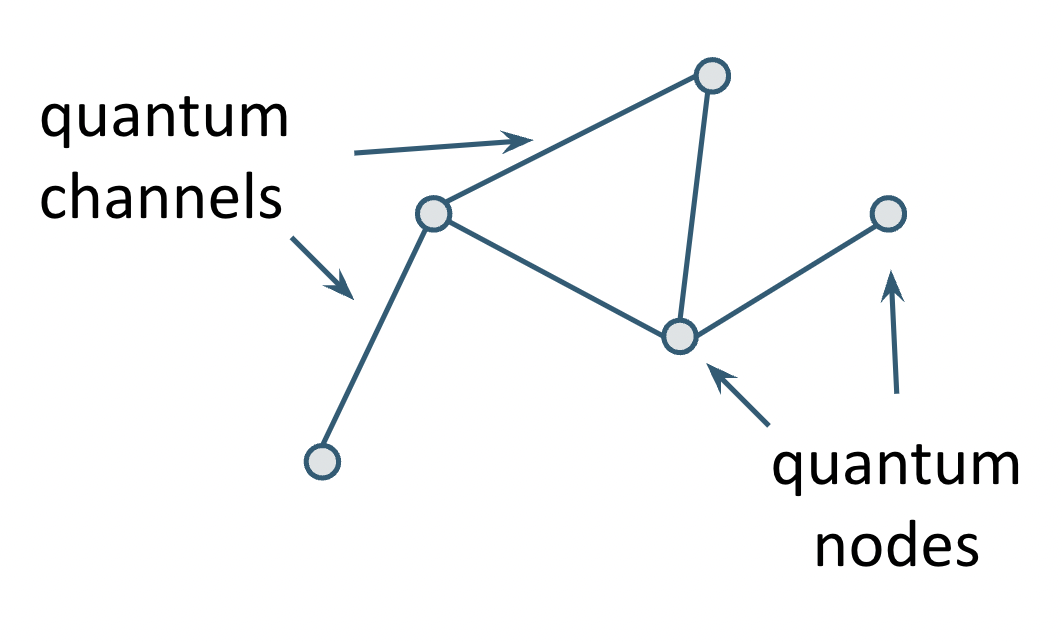
\includegraphics[width=0.8\textwidth]{lesson8/quantum-network.png}
        \caption{A quantum network consists of quantum nodes, and quantum channels that we will call links.}
    \label{fig:quantum-network}
\end{figure}
\begin{figure}[H]
    \centering
    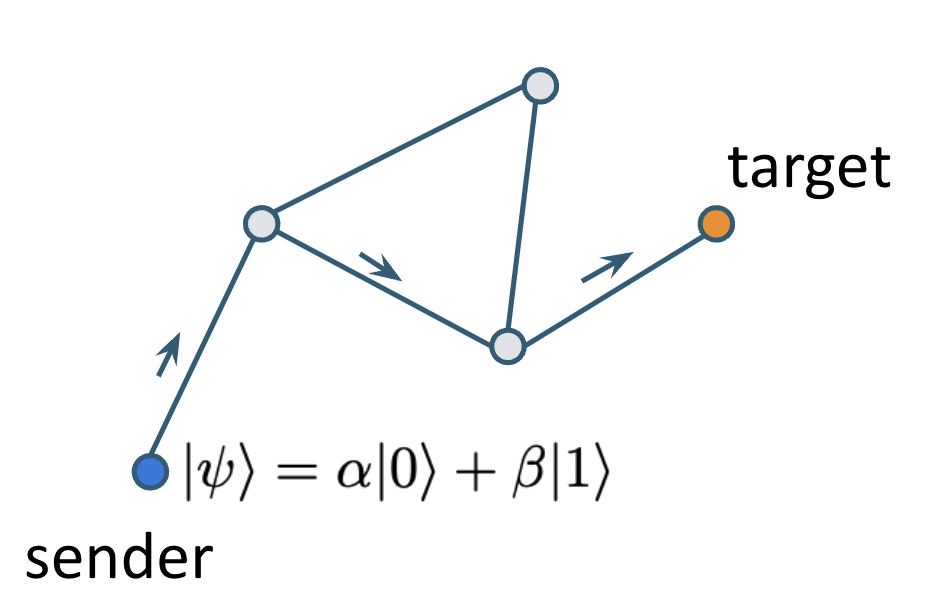
\includegraphics[width=0.8\textwidth]{lesson8/hop-by-hop.png}
        \caption{Physically moving a quantum message}
    \label{fig:hop-by-hop}
\end{figure}
\begin{figure}[H]
    \centering
    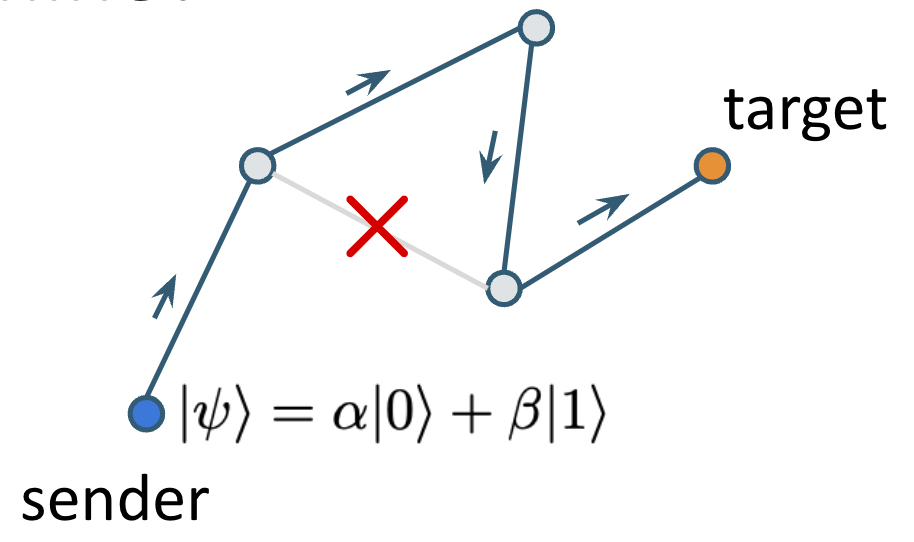
\includegraphics[width=0.8\textwidth]{lesson8/link-down.png}
        \caption{Rerouting when a link goes down.}
    \label{fig:link-down}
\end{figure}
\begin{figure}[H]
    \centering
    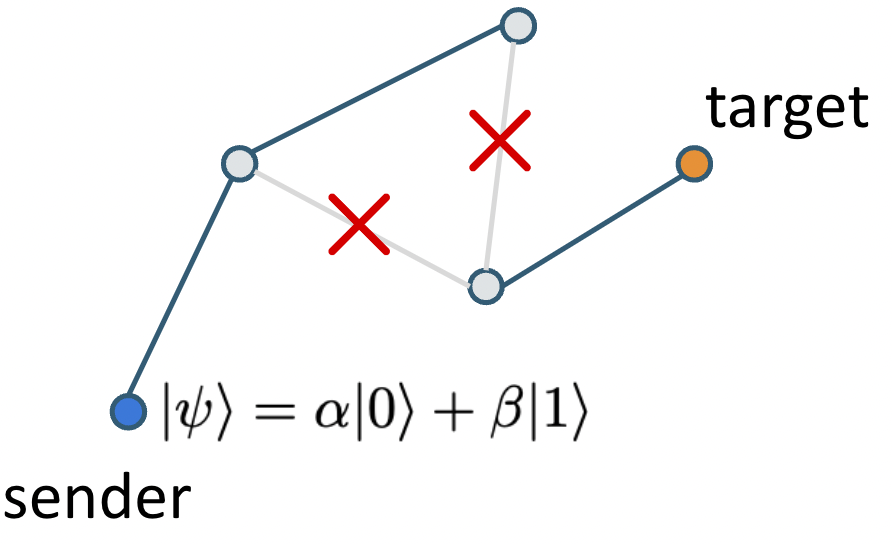
\includegraphics[width=0.8\textwidth]{lesson8/partitioned.png}
        \caption{A partitioned network.}
    \label{fig:partition}
\end{figure}


However in quantum physics, it's a little bit different. We can also transmit the (quantum) message without transmitting the (quantum) physical system. Consider a quantum network like this, \rdv{figure!} and let's say that we want to use the old-fashioned way of transmitting the message with the physical system that is encoding it. In this network, the circles represent our nodes and these lines represent the links or quantum channels between the nodes. The sender, represented by the blue node in the figure, is in possession of some pure state $\ket{psi} = \alpha\ket{0}+\beta\ket{1}$, and  wants to send this state to the target given by the orange network node. The sender can decide (or the network can decide) to send it first to this network node, then to this network node, and then finally to reach the target. But what happens if one of the quantum links is not working? Well, in this particular case, it's not a big problem because the message can be simply rerouted to go around the damaged link and still reach the target. But what happens if another link is down? Well in this case, the network is \emph{partitioned} and it seems like we cannot transmit the message to the target...unless we use teleportation! We can teleport this state from the sender to the target, provided that some initial conditions are met. We can move the information itself without moving the actual physical system. That physical system remains stationary.

\begin{figure}[H]
    \centering
    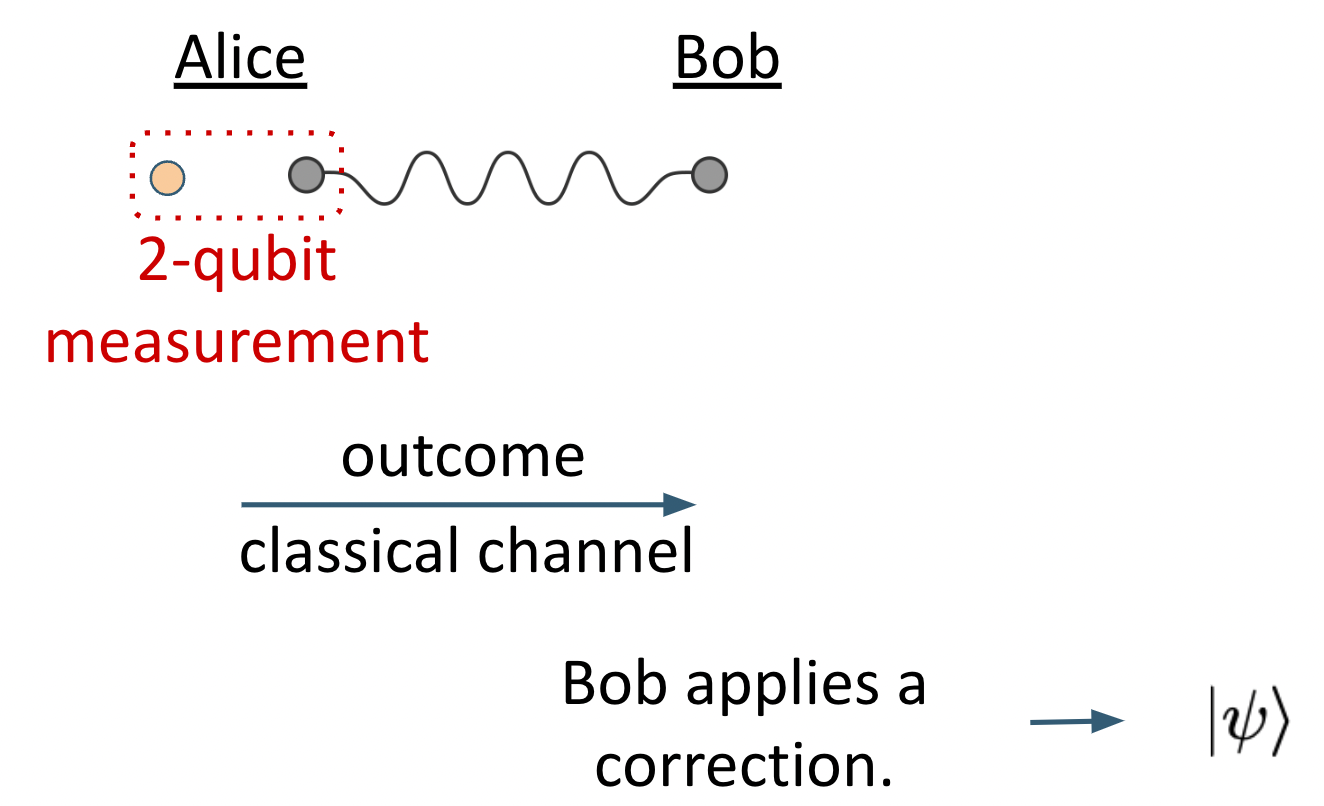
\includegraphics[width=0.8\textwidth]{lesson8/teleportation.png}
        \caption{Teleportation.}
    \label{fig:teleportation}
\end{figure}

This is the outline of the protocol: We will consider our sender and call her "Alice", and she wants to send this quantum state $\ket{\psi}$ to her friend "Bob".  Alice and Bob start by sharing an entangled pair of qubits. Then Alice does a two-qubit measurement on both of her qubits. That measurement provides her with two classical bits, because the measurement is on two qubits.  Naturally, this means that there are four possible outcomes. Alice then communicates this outcome to Bob via a classical channel, and she can do it because the outcome is represented by two classical bits.  Bob then receives this classical message, applies some local corrections, and he ends up with the desired state $\ket{\psi}$.  

Now you see the two conditions necessary to maintain our ability to teleport quantum data even when the quantum network is partitioned: we must have a supply of entanglement, and we must have the ability to exchange classical messages.

\section{Teleportation protocol}

% Step Two: Teleportation Protocol

Let's look at the protocol in more mathematical detail.  First, consider the initial state in our protocol. Alice has an arbitrary qubit given by
\begin{align}
    \ket{\psi} = \alpha\ket{0} + \beta\ket{1}.
\end{align}
Alice and Bob are also sharing an entangled state, and the entire state is given here. It's one of the Bell states- it's $\ket{\Phi^+}$ (phi plus), which is equal superposition of zero zero and one one, and we represent it here on the right as this wavy line, and we are going to label the qubits as follows: A1 is the first qubit of Alice which is her state that she is trying to communicate to Bob. A2 is her second qubit which is one part of the entangled bell pair, and by B we designate Bob's qubit which is part of the entangled pair that he is sharing with Alice.

If we write out the initial state in its full form, it's as follows,
\begin{align}
    \begin{aligned}
|\psi\rangle_{A_{1}}\left|\Phi^{+}\right\rangle_{A_{2} B} &=(\alpha|0\rangle+\beta|1\rangle)_{A_{1}} \frac{1}{\sqrt{2}}(|00\rangle+|11\rangle)_{A_{2} B} \\
&=\frac{1}{\sqrt{2}}(\alpha|000\rangle+\alpha|011\rangle+\beta|100\rangle+\beta|111\rangle)_{A_{1} A_{2} B}
\end{aligned}
\end{align}
it's psi A1 which is Alice's input state that she wants to communicate, and the state phi plus for qubits A2 and B. We can write it out like this, and then expand to get the following superposition of basis states- (zero zero zero), (zero one one), (one zero zero), and (one one one), each with the corresponding probability amplitudes.

Then, we said that Alice performs a Bell basis measurement.

So these are the following bell states- phi plus is given as a superposition of zero zero and one one. Phi minus is this similar superposition between (zero zero) (one one), but now we have a negative phase here. And psi plus is where the qubits are anti-correlated it's (zero one) plus (one zero), and psi minus is (zero one) minus (one zero). And doing a measurement in these Bell basis is basically asking the question: which of these following states is Alice's state in? 
\begin{align}
    \begin{array}{ll}
\left|\Phi^{+}\right\rangle=\frac{1}{\sqrt{2}}(|00\rangle+|11\rangle) & \left|\Phi^{-}\right\rangle=\frac{1}{\sqrt{2}}(|00\rangle-|11\rangle) \\
\left|\Psi^{+}\right\rangle=\frac{1}{\sqrt{2}}(|01\rangle+|10\rangle) & \left|\Psi^{-}\right\rangle=\frac{1}{\sqrt{2}}(|01\rangle-|10\rangle)
\end{array}
\end{align}
So to help us with answering that question, we have to rewrite our initial state in a slightly different form, and to do that we will use the following trick- instead of writing the state zero zero for the two qubits that Alice has, we can write it as a superposition of two of the Bell states, namely zero zero (you can check yourself can be written as superposition of phi plus and phi minus), zero one is then written as a superposition of psi plus and psi minus, and similarly the states one zero and one one can be written as superpositions but with negative phases over there.
\begin{align}
    \begin{array}{ll}
|00\rangle=\frac{1}{\sqrt{2}}\left(\left|\Phi^{+}\right\rangle+\left|\Phi^{-}\right\rangle\right) & |01\rangle=\frac{1}{\sqrt{2}}\left(\left|\Psi^{+}\right\rangle+\left|\Psi^{-}\right\rangle\right) \\
|10\rangle=\frac{1}{\sqrt{2}}\left(\left|\Psi^{+}\right\rangle-\left|\Psi^{-}\right\rangle\right) & |11\rangle=\frac{1}{\sqrt{2}}\left(\left|\Phi^{+}\right\rangle-\left|\Phi^{-}\right\rangle\right)
\end{array}
\end{align}

Let's rewrite Alice's initial state. This is her state, and we are trying to do a two qubit measurement on her qubits.
\begin{align}
    \begin{aligned}
|\psi\rangle_{A_{1}}\left|\Phi^{+}\right\rangle_{A_{2} B} &=(\alpha|0\rangle+\beta|1\rangle)_{A_{1}} \frac{1}{\sqrt{2}}(|00\rangle+|11\rangle)_{A_{2} B} \\
&=\frac{1}{\sqrt{2}}(\alpha|000\rangle+\alpha|011\rangle+\beta|100\rangle+\beta|111\rangle)_{A_{1} A_{2} B}
\end{aligned}
\end{align}

We go term by term, and we first look at Alice's qubit zero zero. We said that that can be rewritten with the help of these following tricks. So we look at zero zero, and we substitute for it our superposition of Bell states- psi plus and psi minus. We do the same thing for the next term in the initial state zero one, and we substitute for it superposition of psi plus and psi minus, and so on and so forth. So in full, what we get is the following superposition- the first term transforms into (alpha times a superposition of Bell state psi plus psi minus times Bob's state zero), and that is in a superposition with this term over here, this third term, and this fourth term.

\begin{align}
    \begin{aligned}
|\psi\rangle_{A_{1}}\left|\Phi^{+}\right\rangle_{A_{2} B} &=(\alpha|0\rangle+\beta|1\rangle)_{A_{1}} \frac{1}{\sqrt{2}}(|00\rangle+|11\rangle)_{A_{2} B} \\
&=\frac{1}{\sqrt{2}}(\alpha|000\rangle+\alpha|011\rangle+\beta|100\rangle+\beta|111\rangle)_{A_{1} A_{2} B} \\
=& \frac{1}{\sqrt{2}}\left(\alpha\left(\left|\Phi^{+}\right\rangle+\left|\Phi^{-}\right\rangle\right)|0\rangle\right.\\
&+\alpha\left(\left|\Psi^{+}\right\rangle+\left|\Psi^{-}\right\rangle\right)|1\rangle \\
&+\beta\left(\left|\Psi^{+}\right\rangle-\left|\Psi^{-}\right\rangle\right)|0\rangle \\
&\left.+\beta\left(\left|\Phi^{+}\right\rangle-\left|\Phi^{-}\right\rangle\right)|1\rangle\right) \\
&=\frac{1}{2}\left|\Phi^{+}\right\rangle_{A_{1} A_{2}}(\alpha|0\rangle+\beta|1\rangle)_{B} \\
&+\frac{1}{2}\left|\Phi^{-}\right\rangle_{A_{1} A_{2}}(\alpha|0\rangle-\beta|1\rangle)_{B} \\
&+\frac{1}{2}\left|\Psi^{+}\right\rangle_{A_{1} A_{2}}(\alpha|1\rangle+\beta|0\rangle)_{B} \\
&+\frac{1}{2}\left|\Psi^{-}\right\rangle_{A_{1} A_{2}}(\alpha|1\rangle-\beta|0\rangle)_{B}
\end{aligned}
\end{align}
Now let's collect all the terms that have the same Bell state for Alice's qubits A1 and A2. So we can see that this term here -this first term has a psi plus that appears in there, and also the last term has a psi plus, but they differ in their amplitudes and also in the state of bob's qubit. So for the first term, we've got probability amplitude alpha and Bob's qubit in the state zero. For the last term, we've got probability amplitude beta and Bob's qubit is in the state one. We collect them together, and what we get is the following expression- we've got psi plus for a state of qubits A1 and A2, so Alice's qubits, and Bob's qubit is in this superposition alpha zero plus beta one. And we do this procedure for all of the other Bell states until we arrive at the following expression. So remember, we're not really doing anything yet we are still dealing with the initial state, we are just rewriting it in a more convenient form. So after rewriting it we get the following superposition- when Alice's two qubits are in state psi plus, then Bob's qubit is in the following superposition of zero and one, and similarly for the other terms. Now we're in a position to answer the question that we asked- in which of the bell states are Alice's two qubits? Well she does the two qubit measurement over here, and what she gets are two classical bits because she's measuring two qubits, therefore there are four possible outcomes for the measurement, which can be encoded into two classical bits. And notice that the probabilities of these outcomes are the same even though Alice's state, this orange state, was in an arbitrary superposition of alpha and beta.
\begin{align}
\operatorname{Prob}\left(\left|\Phi^{\pm}\right\rangle\right)=\operatorname{Prob}\left(\left|\Psi^{\pm}\right\rangle\right)=\frac{1}{4}
\end{align}
The probability of her two-qubit measurement does not depend on these probability amplitudes alpha and beta. All of the outcomes of the Bell state measurement are equal. So the probability of obtaining a phi plus, or a phi minus, or psi plus, or a psi minus, is one quarter.

So, she performs the measurement and the outcome of a measurement determines the state of Bob's qubit. If Alice measures phi plus, then we know that Bob has the desired output state alpha zero plus beta one, which was initial state that Alice was trying to communicate to him. So in that case, we can say, "Great! Our teleportation has succeeded." Bob obtained the state psi.

How about these other cases? Remember we said that all of these outcomes are equally likely, so Alice might get a phi minus or psi plus or psi minus as the outcome of her bell state measurement. In that case, Bob's qubit represents to different states. It does not correspond to the state that Alice was trying to communicate to him given by the state psi.  Summarizing:

\noindent
If Alice measures $\left|\Phi^{+}\right\rangle$, Bob has $\alpha|0\rangle+\beta|1\rangle$.\\
If Alice measures $\left|\Phi^{-}\right\rangle$, Bob has $\alpha|0\rangle-\beta|1\rangle$.\\
If Alice measures $\left|\Psi^{+}\right\rangle$, Bob has $\alpha|1\rangle+\beta|0\rangle$.\\
If Alice measures $\left|\Psi^{-}\right\rangle$, Bob has $\alpha|1\rangle-\beta|0\rangle$.

So what does it mean? Does it mean that our teleportation has failed? No. Luckily, these other states corresponding to the different bell states can be brought into psi by suitable application of a unitary, in particular, notice that if we apply a Pauli Z on the state psi, then we obtain alpha zero minus beta one, which is Bob's state right here. Corresponding to the Bell state psi minus, if we apply X to the state psi, then we get alpha one plus beta zero, which is this state over here. And similarly if we apply the product of X and Z on our initial state psi, then we get alpha one minus beta zero, which is this state over here. 

\begin{align}
\begin{aligned}
|\psi\rangle &=\alpha|0\rangle+\beta|1\rangle \\
Z|\psi\rangle &=\alpha|0\rangle-\beta|1\rangle \\
X|\psi\rangle &=\alpha|1\rangle+\beta|0\rangle \\
X Z|\psi\rangle &=\alpha|1\rangle-\beta|0\rangle
\end{aligned}
\end{align}

So what Alice needs to do is she needs to let Bob know which measurement outcome she obtained, and she does it by sending two classical bits. And then Bob knows exactly which correction he has to apply. If Alice measures phi plus, he does nothing because he already has the state psi. If Alice measures phi minus, then Bob knows he has to apply a Pauli Z to his qubit. If she tells him that she obtained the measurement outcome psi plus, he simply applies Pauli X, and if she obtains a psi minus then he just needs to apply Z times X to his qubit.  Summarizing,

\noindent
If Alice measures $\left|\Phi^{+}\right\rangle$, Bob applies $I$.\\
If Alice measures $\left|\Phi^{-}\right\rangle$, Bob applies $Z$.\\
If Alice measures $\left|\Psi^{+}\right\rangle$, Bob applies $X$.\\
If Alice measures $\left|\Psi^{-}\right\rangle$, Bob applies $Z X$.

And in all of these cases, Bob ends up with the desired state $\ket{psi}$, so our teleportation has succeeded and Alice managed to communicate her state $\ket{\psi}$ to Bob without actually sending it through the network. That's amazing!

Also, one thing that teleportation demonstrates is the interchangeability of resources in quantum communication and also quantum computation. In here the different resources are the following- we have exchanged one qubit of communication for one entangled pair and two classical bits. What does it mean? It means that we achieved the task of sending the information about state psi from Alice to Bob by two different ways. We could have just send it directly, which is considered as one qubit of communication. That will definitely get the state from Alice to Bob. Or- as we outlined with the teleportation protocol, rather than sending the state directly, if Alice and Bob share an entangled pair, "and" are allowed to communicate two classical bits, then they can achieve the same task.

\section{No-cloning theorem and FTL communication}

Step three: No-cloning Theorem and Faster-than-light (FTL) Communication

So, let's go back to the teleportation protocol and ask a few questions. Alice communicated her state to Bob. Did she clone it while teleporting it? After all she started with the state psi and she did not send the physical qubit to Bob. Yet at the end of the protocol, we saw that Bob does have the qubit psi. So what was going on there? Well initially Bob's qubit was part of a maximally entangled state. He had one part of the entangled state and Alice had the other. At the end of the protocol Alice's qubit A1 was part of a maximally entangled state. She performed a measurement in the Bell basis and that projected her two qubits onto one of the four possible Bell states where all of them are maximally entangled. So what that means is that initially the state of the qubit A1 was psi, and the state of the qubit that Bob had in his possession was a maximally mixed state, and then after the protocol the state of Alice's qubit A1 became the maximally mixed state, whereas Bob's qubit became the state psi. So we see that there was no cloning or copying of the state even though there was no direct physical transmission of the state psi from Alice to Bob. But this is an interesting question- "is cloning possible?" And let's have a look at it.

So let's only consider cloning of pure states, and let's say that we've got some device. This is our hypothetical cloning device, and how it works is that it's some unitary, and the input states is some arbitrary state psi with some other state which is initialized in state zero. So it's a two qubit input state and we've got a two qubit output state where both of the qubits are now in the state psi. Now the question that we are trying to answer- is such a transformation possible? What does the unitary look like that can achieve such a transformation?

For example if we start in the state zero zero, after applying our cloning unitary we would like to obtain state zero zero. That makes sense. If we start in the state plus zero and apply our cloning unitary, we would like to obtain as output states, plus for the first qubit and plus for the second qubit, and so on and so forth until it works for a general input state.

So before we present a proof of what's going on, let's consider some examples to get some intuition.

And let's consider a CNOT gate as our unitary U. So a CNOT gate is represented here in the Dirac notation, or here in the matrix notation. What this really means is that if the state of the first qubit is zero, then apply the identity to the second qubit, meaning "don't do anything". If the state of the first qubit is one, then apply Pauli X to the second qubit.

And let's consider some inputs. So first, let's try a very simple input zero zero. If we apply CNOT, you can check for yourself the output is also zero zero. So in this case, we can say that we have cloned the qubit even though we haven't really done anything. Second case is more interesting. We start in the state one zero. So now, we are trying to clone the state one, and as we said if the state of the first qubit is one, we apply the Pauli X to the second qubit, and in fact our input state is in one and our second state is a zero, but after application of the Pauli X it flips into one. So we went from input one zero to output one one. So again, we have cloned our state. How about if we consider a superposition of zero and one as our input? So, our total input is psi zero. In this case, if you apply the unitary CNOT, you will see that you obtain an entangled state zero zero plus one one, which is not the product state that we were aiming for. We were aiming for plus plus. So in this case cloning has failed, at least with this example of CNOT and this particular input.

So, let's look at the cases when it worked and then when it didn't. It worked when we were trying to clone the state zero and the state one, but it failed when we were trying to clone some superposition of these two states. So it appears that we can only clone states which are orthogonal. Well, let's try and prove it.

Let's say that we are trying to clone an arbitrary state psi, so our expected or our desired output is psi psi.

And let's say that it works for any two input states. So it doesn't matter if our input is psi or some other general state phi. We require from our cloning device that it works in any scenario. So in the first case when our input set is psi, our output is psi psi, whereas in the second case when our input is phi, our output is phi phi. Now what we can do is we can take these two expressions and we can take the inner product of the left hand sides and the right hand sides of these two expressions. So on the right hand side is quite simple, we take the inner product of phi of the first qubit with psi of the first qubit, and we multiply it by the inner product of this second phi and this second psi, so we get the inner product of phi psi squared. Whereas here on this side, we've got these unitaries. What actually happens when we take the inner product, the second unitary turns into a U-dagger, and we know that one of the defining properties of a unitary is that U-dagger times U is equal to identity. So, these unitaries cancel, and what we get is the inner product of phi and psi, multiplied by the inner product of zero and zero. But we know what the inner product of zero zero is- it's just one. So on the left hand side, we end up with just the inner product of phi and psi, and that has to be equal to the same inner product squared. So we can now easily solve for what the inner product between these two arbitrary states should be. Well, in order to satisfy this equation it has to be zero or it has to be one. So what does this actually mean? When the inner product of two states is one, it means that the two states are actually only one state. They must be the same because we assume that they are normalized, as all states should be. On the other hand when it's zero, it means that the two states are orthogonal. So our cloning really works, as we saw in the example before, for states that can be distinguished with certainty. Remember, orthogonal states are always distinguishable deterministically. So we can say that no-cloning for arbitrary states- we cannot clone an arbitrary state in quantum mechanics, which is in stark contrast to classical physics. Now let's ask a second interesting question- is teleportation instantaneous? Can we communicate faster than the speed of light? And in order to answer that question we have to consider the timeline of events that are going on during our teleportation protocol. So this is our timeline, and we start at time t0, when we initialize our system. So this is when we create our initial state. At some later time t1, Alice performs her measurement in the Bell basis on the two qubits that she has. Then at some later time t2, Alice sends the outcome of the measurements to Bob, and he receives these outcomes at time t3, so let's go step by step and consider what is going on with Bob's state. So at time t0, we said that Bob's qubit is part of a maximally entangled pair, which means that the reduced density of his qubit is a maximally mixed state, meaning if he measures it in Pauli Z basis, he will get the outcome zero with probability half, or the outcome one with probability half. In fact, if he measures in any basis, he will get the outcome plus one or minus one with the same probability, so he's maximally unsure about his own state. That also means that he has no idea about Alice's state.

Then at time t1, Alice performs her measurement. So just before the measurement, the total state of all three qubits is given by this expression which we derived in the previous step. So we can rewrite the initial state in terms of the Bell basis for Alice's qubits, which leaves Bob's qubit in these following states depending on which state Alice has. So at this time does Bob know anything about Alice's state A1? He doesn't, because nothing really happened. We have only rewritten the initial state. So, above state is still maximally mixed we. Then we ask the question- what happens just after t1, just after Alice measures in the Bell basis? So just after the measurement, he knows that with probability one quarter, Alice measured the outcome phi plus, and with the same probability she could have obtained the other three remaining Bell states. So he knows that with probability one quarter, he has the state psi, or with probability one quarter he has some equivalent state given by these following expressions. And this is a distribution which we can write in the density matrix formalism, so let's do that. Bob's qubit can be written as follows- with probability a quarter, he has the state alpha zero plus beta one, which in density matrix formalism is given by the outer product. With probability one quarter, here's the following state, and so on and so forth for the other two possibilities. We can go through the algebra and we will see that the cross terms cancel, and in fact what we obtain is that the state of Bob, given by "rho B", is this expression right here which can simplify to, again, a maximally mixed state. This is because we started with state psi which is normalized, meaning mod alpha squared plus mod beta squared has to be equal to one. So even just after the measurement, Bob still doesn't know anything about the state psi, his qubit is maximally mixed. Let's see what happens when we go to time t2. At this time, we say that Alice sends the outcome to Bob. Well, nothing really changes from just after the measurement occurred at time t1, because Bob has not received the message about the outcomes of the measurements, so his state is still maximally mixed state. He has no information about the state to be teleported, state psi. So still no teleportation, even though the measurement by Alice has been performed at time t1. Finally at time t3, Bob receives Alice's message, he receives the two qubits telling him about which outcome she measured.

And then Bob finally has the following state- he has the state psi up to some unitary, Pauli X, Y, or the product of X and Y. So it's only at this time, at time t3, when he receives the message that teleportation really, truly, has taken place. Bob must receive the classical message in order for teleportation to work, so he has to wait all this time from t2 to t3 to receive this message, and this message can travel maximally at the speed of light. So we don't communicate faster than the speed of light and we do not violate special relativity.


\section{Simulating teleportation}

(Hands-on exercises for simulating teleportation to be added as a Jupyter Qiskit notebook.)


\newpage
\begin{exercises}
\exer{Consider the following quantum state:}
\begin{equation*}
\ket{\psi} = \frac{\sqrt{3}}{2}\ket{0} + \frac{1}{2}\ket{1}
\end{equation*}
\subexer{Find the probability of measuring a zero.}
\subexer{Find the probability of measuring a one.}


\end{exercises}

